\documentclass[aspectratio=169, 10pt]{beamer}

% ==============================================================================
% Packages & Professional Academic Typography
% ==============================================================================
\usepackage[utf8]{inputenc}
\usepackage[T1]{fontenc}
\usepackage{lmodern}
\usepackage{microtype}
\usepackage{booktabs}
\usepackage{array}
\usepackage{amsmath,amssymb}
\usepackage[most]{tcolorbox}
\usepackage{tikz}
\usetikzlibrary{automata, positioning, arrows.meta, shapes.geometric, calc, fit}

% ==============================================================================
% Design System & Refined Academic Color Palette (GIMPA Branding)
% ==============================================================================
\definecolor{gimpanavy}{RGB}{10, 37, 64}       % #0A2540 Deep Academic Navy
\definecolor{gimpaslate}{RGB}{51, 65, 85}      % #334155 Slate Gray
\definecolor{gimpaaccent}{RGB}{30, 107, 184}   % #1E6BB8 Scholarly Blue
\definecolor{charcoalText}{RGB}{30, 41, 59}     % #1E293B High-contrast body
\definecolor{lightBg}{RGB}{248, 250, 252}      % #F8FAFC Clean card background
\definecolor{ruleGray}{RGB}{226, 232, 240}     % #E2E8F0 Subtle divider
\definecolor{accentCrimson}{RGB}{185, 28, 28}  % #B91C1C Academic Alert
\definecolor{accentGreen}{RGB}{21, 128, 61}    % #15803D Success / Verification
\definecolor{accentAmber}{RGB}{180, 83, 9}     % #B45309 Amber Warning / Key Insight

% Beamer General Settings
\setbeamertemplate{navigation symbols}{}
\setbeamercolor{background canvas}{bg=white}
\setbeamercolor{normal text}{fg=charcoalText}
\setbeamercolor{structure}{fg=gimpanavy}
\setbeamercolor{title}{fg=gimpanavy}
\setbeamercolor{author}{fg=gimpaslate}
\setbeamercolor{institute}{fg=gimpaslate}
\setbeamercolor{date}{fg=gimpaslate}

% Clean, Dignified Frametitle
\setbeamertemplate{frametitle}{
  \vspace{0.12cm}
  \noindent
  {\large\bfseries\color{gimpanavy}\insertframetitle}
  \ifx\insertframesubtitle\@empty\else
    \\[0.03cm]{\footnotesize\color{gimpaslate}\insertframesubtitle}
  \fi
  \vspace{0.04cm}
  {\color{ruleGray}\hrule height 0.6pt}
  \vspace{0.05cm}
}

% Sleek Minimalist Footline
\setbeamertemplate{footline}{
  \vspace{-0.40cm}
  \begin{center}
    {\color{ruleGray}\rule{0.95\paperwidth}{0.5pt}}
  \end{center}
  \vspace{-0.15cm}
  \leavevmode%
  \hbox{%
    \begin{beamercolorbox}[wd=0.45\paperwidth,ht=2.5ex,dp=1.2ex,left]{footline}%
      \hspace*{0.6cm}{\scriptsize\color{gimpaslate}\textbf{CS 305: Theory of Computation} \;\textbar\; Week 2}
    \end{beamercolorbox}%
    \begin{beamercolorbox}[wd=0.33\paperwidth,ht=2.5ex,dp=1.2ex,center]{footline}%
      {\scriptsize\color{gimpaslate}GIMPA School of Technology}
    \end{beamercolorbox}%
    \begin{beamercolorbox}[wd=0.22\paperwidth,ht=2.5ex,dp=1.2ex,right]{footline}%
      {\scriptsize\color{gimpaslate}\insertframenumber{} / \inserttotalframenumber}\hspace*{0.6cm}
    \end{beamercolorbox}%
  }%
  \vspace*{0.20cm}
}

% Minimalist Square Bullets
\setbeamertemplate{itemize item}{{\color{gimpaaccent}\scriptsize$\blacksquare$}}
\setbeamertemplate{itemize subitem}{{\color{gimpaslate}\tiny$\blacktriangleright$}}
\setbeamertemplate{enumerate item}{\textbf{\color{gimpanavy}\insertenumlabel.}}

% ==============================================================================
% Card Environments & Section Styling
% ==============================================================================
\newcommand{\colheader}[1]{%
  {\noindent\footnotesize\bfseries\color{gimpanavy}#1}%
  \vspace{0.02cm}%
  {\color{gimpanavy!30}\hrule height 0.5pt}%
  \vspace{0.05cm}%
}

\newcommand{\cardtitle}[1]{{\noindent\footnotesize\bfseries\color{gimpanavy}#1}\par\vspace{0.03cm}}
\newcommand{\alerttitle}[1]{{\noindent\footnotesize\bfseries\color{accentCrimson}#1}\par\vspace{0.03cm}}
\newcommand{\ambertitle}[1]{{\noindent\footnotesize\bfseries\color{accentAmber}#1}\par\vspace{0.03cm}}
\newcommand{\greentitle}[1]{{\noindent\footnotesize\bfseries\color{accentGreen}#1}\par\vspace{0.03cm}}

\tcbset{
  before=\vspace{1pt},
  after=\vspace{1pt},
  top=2.5pt,
  bottom=2.5pt,
  left=5pt,
  right=5pt,
  boxrule=0.5pt,
  arc=2pt,
  conceptcard/.style={
    enhanced,
    colback=lightBg,
    colframe=ruleGray,
    borderline west={2.5pt}{0pt}{gimpanavy}
  },
  examplecard/.style={
    enhanced,
    colback=lightBg,
    colframe=ruleGray,
    borderline west={2.5pt}{0pt}{accentGreen}
  },
  alertcard/.style={
    enhanced,
    colback=lightBg,
    colframe=ruleGray,
    borderline west={2.5pt}{0pt}{accentCrimson}
  },
  spotlightcard/.style={
    enhanced,
    colback=gimpaaccent!5,
    colframe=ruleGray,
    borderline west={2.5pt}{0pt}{gimpaaccent}
  },
  quizcard/.style={
    enhanced,
    colback=accentAmber!5,
    colframe=ruleGray,
    borderline west={2.5pt}{0pt}{accentAmber}
  }
}

% TikZ Automata Settings
\tikzset{
  every state/.style={
    draw=gimpanavy,
    thick,
    fill=white,
    minimum size=7.5mm,
    inner sep=1pt,
    font=\small\bfseries\color{gimpanavy}
  },
  initial text={},
  initial distance=5mm,
  every initial by arrow/.style={
    ->,
    >=stealth,
    thick,
    draw=gimpanavy
  },
  accepting/.style={
    double,
    double distance=1.5pt,
    thick,
    draw=gimpanavy
  },
  every edge/.style={
    ->,
    >=stealth,
    thick,
    draw=gimpanavy,
    font=\footnotesize
  }
}

% ==============================================================================
% Course & Presentation Metadata
% ==============================================================================
\title{\textbf{\LARGE Deterministic Finite Automata (DFA)}}
\subtitle{\vspace{0.12cm}\large Week 2: Formal 5-Tuples, State Diagrams, Closure Proofs, and Line-Rate DPI}
\author{\textbf{School of Technology}}
\institute{Ghana Institute of Management and Public Administration (GIMPA)}
\date{Academic Year 2026/2027}

\begin{document}

% ------------------------------------------------------------------------------
% SLIDE 1: Title Slide
% ------------------------------------------------------------------------------
\begin{frame}[plain]
  \vspace{0.4cm}
  \begin{center}
    {\scriptsize\bfseries\color{gimpaaccent}CS 305: THEORY OF COMPUTATION --- WEEK 2 LECTURE}\\[0.22cm]
    {\LARGE\bfseries\color{gimpanavy}Deterministic Finite Automata\\[0.08cm] (DFA)}\\[0.22cm]
    {\normalsize\color{gimpaslate}Formal 5-Tuples, State Diagrams, Product Construction \& Line-Rate Packet Filtering}\\[0.30cm]
    
    {\color{ruleGray}\rule{0.6\paperwidth}{0.6pt}}\\[0.30cm]
    
    {\small\bfseries\color{gimpanavy}School of Technology}\\[0.06cm]
    {\footnotesize\color{gimpaslate}Ghana Institute of Management and Public Administration (GIMPA)}\\[0.20cm]
    {\scriptsize\color{gimpaslate}Textbook Reference: Michael Sipser, \textit{Introduction to the Theory of Computation} (3rd Ed.), Section 1.1}
  \end{center}
\end{frame}

% ------------------------------------------------------------------------------
% SLIDE 2: Week 1 Recap & Lecture Roadmap
% ------------------------------------------------------------------------------
\begin{frame}{Week 1 Recap \& Week 2 Roadmap}
  \framesubtitle{Transitioning from informal mathematical foundations to rigorous machine models}
  
  \begin{columns}[T]
    \begin{column}{0.48\textwidth}
      \colheader{Week 1 Foundations Recap}
      \begin{tcolorbox}[conceptcard]
        \cardtitle{What We Established:}
        \begin{itemize}\setlength{\itemsep}{2pt}\scriptsize
          \item \textbf{Alphabets ($\Sigma$):} Non-empty finite sets of symbols.
          \item \textbf{Strings ($w \in \Sigma^*$):} Finite sequences of symbols, length $|w|$, empty string $\varepsilon$.
          \item \textbf{Languages ($L \subseteq \Sigma^*$):} Formal decision problems.
          \item \textbf{Chomsky Type 3:} The class of regular languages recognizes patterns with $\mathcal{O}(1)$ constant memory.
        \end{itemize}
      \end{tcolorbox}
    \end{column}
    
    \begin{column}{0.48\textwidth}
      \colheader{Today's Agenda (Week 2)}
      \begin{tcolorbox}[spotlightcard]
        \cardtitle{Core Topics Today:}
        \begin{itemize}\setlength{\itemsep}{2pt}\scriptsize
          \item \textbf{Formal 5-Tuple Definition:} $M = (Q, \Sigma, \delta, q_0, F)$.
          \item \textbf{DFA Design Patterns:} Substring search, modulo counting, and binary divisibility.
          \item \textbf{Formal Computation \& Extended $\delta^*$:} Exact acceptance conditions.
          \item \textbf{Closure Proofs:} Product construction for Union ($\cup$) and Intersection ($\cap$).
          \item \textbf{Systems Spotlight:} Line-rate 100 Gbps Deep Packet Inspection (Snort/Zeek).
        \end{itemize}
      \end{tcolorbox}
    \end{column}
  \end{columns}
  
  \vspace{0.08cm}
  \begin{tcolorbox}[alertcard]
    {\scriptsize\textbf{Pedagogical Milestone:} Today we assign \textbf{Problem Set 1} (due Week 3), focusing on formal DFA constructions and closure property proofs.}
  \end{tcolorbox}
\end{frame}

% ------------------------------------------------------------------------------
% SLIDE 3: Formal Definition of a DFA
% ------------------------------------------------------------------------------
\begin{frame}{Formal Definition of a DFA}
  \framesubtitle{Michael Sipser, Definition 1.5: The 5-tuple mathematical foundation}
  
  \begin{columns}[T]
    \begin{column}{0.50\textwidth}
      \colheader{The 5-Tuple Specification}
      \begin{tcolorbox}[conceptcard]
        \cardtitle{Definition 2.1: DFA 5-Tuple}
        {\scriptsize
        A \textbf{Deterministic Finite Automaton} (DFA) is a 5-tuple:
        \[ M = \bigl(Q, \Sigma, \delta, q_0, F\bigr) \]
        where:
        \begin{enumerate}\setlength{\itemsep}{2pt}\scriptsize
          \item $Q$ is a finite set of \textbf{states}.
          \item $\Sigma$ is a finite set called the \textbf{alphabet}.
          \item $\delta: Q \times \Sigma \to Q$ is the \textbf{transition function}.
          \item $q_0 \in Q$ is the \textbf{start (initial) state}.
          \item $F \subseteq Q$ is the set of \textbf{accept (final) states}.
        \end{enumerate}
        }
      \end{tcolorbox}
    \end{column}
    
    \begin{column}{0.46\textwidth}
      \colheader{What Makes It ``Deterministic''?}
      \begin{tcolorbox}[alertcard]
        \alerttitle{Crucial Deterministic Invariants}
        \begin{itemize}\setlength{\itemsep}{2.5pt}\scriptsize
          \item \textbf{Total Function:} For \textit{every} state $q \in Q$ and \textit{every} symbol $a \in \Sigma$, $\delta(q, a)$ must specify \textbf{exactly one} next state.
          \item \textbf{No Choices / No Guessing:} The machine's path on any input string $w$ is uniquely determined.
          \item \textbf{No $\varepsilon$-Transitions:} The DFA cannot change state without consuming an input symbol from $\Sigma$.
        \end{itemize}
      \end{tcolorbox}
    \end{column}
  \end{columns}
  
  \vspace{0.08cm}
  \begin{tcolorbox}[spotlightcard]
    {\scriptsize\textbf{State Meaning:} Each state in $Q$ represents an \textbf{equivalence class of past inputs} that require identical future treatment.}
  \end{tcolorbox}
\end{frame}

% ------------------------------------------------------------------------------
% SLIDE 4: Representing DFAs: Diagrams vs Transition Tables
% ------------------------------------------------------------------------------
\begin{frame}{Representing DFAs: Diagrams vs. Transition Tables}
  \framesubtitle{Two isomorphic representations of the transition function $\delta$}
  
  \begin{columns}[T]
    \begin{column}{0.50\textwidth}
      \colheader{Visual State Diagram}
      \begin{center}
        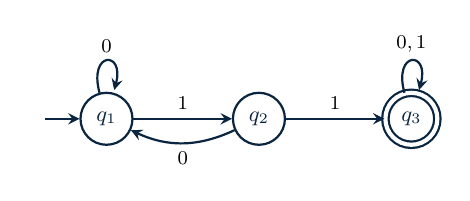
\begin{tikzpicture}[scale=0.88, every node/.style={transform shape}]
          \node[state, initial] (q1) at (0, 0) {$q_1$};
          \node[state] (q2) at (2.2, 0) {$q_2$};
          \node[state, accepting] (q3) at (4.4, 0) {$q_3$};
          
          \path (q1) edge[loop above] node{$0$} (q1)
                (q1) edge node[above]{$1$} (q2)
                (q2) edge[bend left=25] node[below]{$0$} (q1)
                (q2) edge node[above]{$1$} (q3)
                (q3) edge[loop above] node{$0, 1$} (q3);
        \end{tikzpicture}
      \end{center}
      \begin{tcolorbox}[conceptcard]
        \cardtitle{State Semantics:}
        \begin{itemize}\setlength{\itemsep}{1.5pt}\scriptsize
          \item $q_1$: Have not seen a $1$ / last symbol was $0$.
          \item $q_2$: Just read a single $1$.
          \item $q_3$: Have seen substring $11$ (Accepting Sink).
        \end{itemize}
      \end{tcolorbox}
    \end{column}
    
    \begin{column}{0.46\textwidth}
      \colheader{Formal Transition Table ($\delta$)}
      \vspace{0.05cm}
      \begin{center}
        \scriptsize
        \renewcommand{\arraystretch}{1.25}
        \begin{tabular}{@{} c | c c @{}}
          \toprule
          \textbf{State} $q \in Q$ & \textbf{Input} $0$ & \textbf{Input} $1$ \\
          \midrule
          $\to q_1$ & $q_1$ & $q_2$ \\
          $q_2$     & $q_1$ & $q_3$ \\
          $* q_3$   & $q_3$ & $q_3$ \\
          \bottomrule
        \end{tabular}
      \end{center}
      \vspace{0.08cm}
      \begin{tcolorbox}[examplecard]
        \greentitle{Formal Specification of $M_1$:}
        {\scriptsize
        $M_1 = \bigl(\{q_1, q_2, q_3\}, \{0, 1\}, \delta, q_1, \{q_3\}\bigr)$\par
        \textbf{Language Recognized:}
        \[ L(M_1) = \{w \in \{0, 1\}^* \mid w \text{ contains substring } 11\} \]
        }
      \end{tcolorbox}
    \end{column}
  \end{columns}
\end{frame}

% ------------------------------------------------------------------------------
% SLIDE 5: DFA Design Pattern 1: Tracking Substrings
% ------------------------------------------------------------------------------
\begin{frame}{DFA Design Pattern 1: Tracking Substrings}
  \framesubtitle{Methodology: Building progress chains with corrective fallback transitions}
  
  \begin{columns}[T]
    \begin{column}{0.44\textwidth}
      \colheader{Design Objective: Substring ``010''}
      \begin{tcolorbox}[conceptcard]
        \cardtitle{Target Language:}
        {\scriptsize
        $L = \{w \in \{0, 1\}^* \mid w \text{ contains substring } 010\}$
        \vspace{0.04cm}
        
        \textbf{State Meaning Formulation:}
        \begin{itemize}\setlength{\itemsep}{1.5pt}\scriptsize
          \item $q_0$: Matched prefix $\varepsilon$ (no progress).
          \item $q_1$: Matched prefix \texttt{0}.
          \item $q_2$: Matched prefix \texttt{01}.
          \item $q_3$: Matched \texttt{010} (Accepting trap state).
        \end{itemize}
        }
      \end{tcolorbox}
    \end{column}
    
    \begin{column}{0.52\textwidth}
      \colheader{State Diagram with Fallback Arcs}
      \begin{center}
        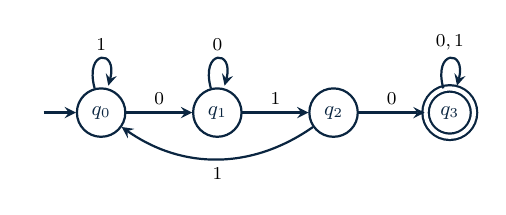
\begin{tikzpicture}[scale=0.82, every node/.style={transform shape}]
          \node[state, initial] (q0) at (0, 0) {$q_0$};
          \node[state] (q1) at (1.8, 0) {$q_1$};
          \node[state] (q2) at (3.6, 0) {$q_2$};
          \node[state, accepting] (q3) at (5.4, 0) {$q_3$};
          
          \path (q0) edge[loop above] node{$1$} (q0)
                (q0) edge node[above]{$0$} (q1)
                (q1) edge[loop above] node{$0$} (q1)
                (q1) edge node[above]{$1$} (q2)
                (q2) edge[bend left=35] node[below]{$1$} (q0)
                (q2) edge node[above]{$0$} (q3)
                (q3) edge[loop above] node{$0, 1$} (q3);
        \end{tikzpicture}
      \end{center}
      \begin{tcolorbox}[examplecard]
        \greentitle{Crucial Fallback Transition Analysis:}
        {\scriptsize
        If in $q_2$ (seen \texttt{01}) we read $1 \implies$ string ends in \texttt{011}. Longest prefix of \texttt{010} in suffix is $\varepsilon \implies$ fallback to $q_0$!
        }
      \end{tcolorbox}
    \end{column}
  \end{columns}
  
  \vspace{0.08cm}
  \begin{tcolorbox}[spotlightcard]
    {\scriptsize\textbf{Pattern Rule:} On mismatch, transition to the state representing the \textbf{longest prefix} of the target pattern that matches the current suffix.}
  \end{tcolorbox}
\end{frame}

% ------------------------------------------------------------------------------
% SLIDE 6: DFA Design Pattern 2: Parity & Counting
% ------------------------------------------------------------------------------
\begin{frame}{DFA Design Pattern 2: Parity \& Modulo Counting}
  \framesubtitle{Tracking independent modular invariants via Cartesian state product}
  
  \begin{columns}[T]
    \begin{column}{0.48\textwidth}
      \colheader{Design Objective: Dual Parity}
      \begin{tcolorbox}[conceptcard]
        \cardtitle{Target Language:}
        {\scriptsize
        $L = \{w \in \{0, 1\}^* \mid w \text{ has even 0s and odd 1s}\}$
        \vspace{0.04cm}
        
        \textbf{Decomposing Invariants:}
        \begin{itemize}\setlength{\itemsep}{2pt}\scriptsize
          \item Number of $0$s mod 2: $\{\text{Even}, \text{Odd}\}$ ($2$ states).
          \item Number of $1$s mod 2: $\{\text{Even}, \text{Odd}\}$ ($2$ states).
          \item Total States: $2 \times 2 = 4$ composite states.
        \end{itemize}
        }
      \end{tcolorbox}
      \begin{tcolorbox}[examplecard]
        \greentitle{State Labeling:}
        {\scriptsize
        $q_{ee}$: (Even 0s, Even 1s) --- Start State\par
        $q_{eo}$: (Even 0s, Odd 1s) --- \textbf{Accept State}\par
        $q_{oe}$: (Odd 0s, Even 1s)\par
        $q_{oo}$: (Odd 0s, Odd 1s)
        }
      \end{tcolorbox}
    \end{column}
    
    \begin{column}{0.48\textwidth}
      \colheader{4-State Parity Diamond}
      \begin{center}
        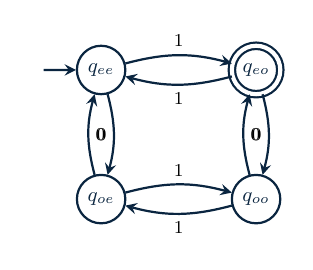
\begin{tikzpicture}[scale=0.82, every node/.style={transform shape}]
          \node[state, initial] (qee) at (0, 2.0) {$q_{ee}$};
          \node[state, accepting] (qeo) at (2.4, 2.0) {$q_{eo}$};
          \node[state] (qoe) at (0, 0) {$q_{oe}$};
          \node[state] (qoo) at (2.4, 0) {$q_{oo}$};
          
          \path (qee) edge[bend left=15] node[above]{$1$} (qeo)
                (qeo) edge[bend left=15] node[below]{$1$} (qee)
                (qoe) edge[bend left=15] node[above]{$1$} (qoo)
                (qoo) edge[bend left=15] node[below]{$1$} (qoe)
                (qee) edge[bend left=15] node[left]{$0$} (qoe)
                (qoe) edge[bend left=15] node[right]{$0$} (qee)
                (qeo) edge[bend left=15] node[left]{$0$} (qoo)
                (qoo) edge[bend left=15] node[right]{$0$} (qeo);
        \end{tikzpicture}
      \end{center}
      \begin{tcolorbox}[spotlightcard]
        {\scriptsize\textbf{Modular Memory Rule:} Any modulo counting $\pmod k$ requires exactly $k$ states. A DFA can count $\pmod k$ for any fixed $k$, but cannot count to infinity.}
      \end{tcolorbox}
    \end{column}
  \end{columns}
\end{frame}

% ------------------------------------------------------------------------------
% SLIDE 7: DFA Design Pattern 3: Binary Divisibility
% ------------------------------------------------------------------------------
\begin{frame}{DFA Design Pattern 3: Binary Divisibility by 3}
  \framesubtitle{Arithmetic stream processing: Updating numerical values on the fly}
  
  \begin{columns}[T]
    \begin{column}{0.48\textwidth}
      \colheader{Mathematical Invariant}
      \begin{tcolorbox}[conceptcard]
        \cardtitle{Language Specification:}
        {\scriptsize
        $L_{\text{div3}} = \{w \in \{0, 1\}^* \mid \text{val}(w) \text{ is divisible by } 3\}$\par
        \textbf{Examples in $L$:} $0$ ($0$), $11$ ($3$), $110$ ($6$), $1001$ ($9$).
        \vspace{0.06cm}
        
        \textbf{Value Recurrence Relation:}
        When appending bit $b \in \{0, 1\}$ to binary string $w$:
        \[ \text{val}(wb) \equiv 2 \cdot \text{val}(w) + b \pmod 3 \]
        \[ \delta(q_r, b) = q_{(2r + b) \bmod 3} \]
        }
      \end{tcolorbox}
    \end{column}
    
    \begin{column}{0.48\textwidth}
      \colheader{3-State Remainder Machine}
      \begin{center}
        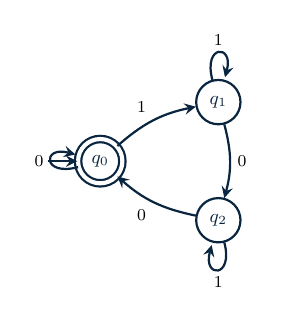
\begin{tikzpicture}[scale=0.75, every node/.style={transform shape}]
          \node[state, initial, accepting] (q0) at (0, 0) {$q_0$};
          \node[state] (q1) at (2.0, 1.0) {$q_1$};
          \node[state] (q2) at (2.0, -1.0) {$q_2$};
          
          \path (q0) edge[loop left] node{$0$} (q0)
                (q0) edge[bend left=15] node[above left]{$1$} (q1)
                (q1) edge[bend left=15] node[right]{$0$} (q2)
                (q1) edge[loop above] node{$1$} (q1)
                (q2) edge[bend left=15] node[below left]{$0$} (q0)
                (q2) edge[loop below] node{$1$} (q2);
        \end{tikzpicture}
      \end{center}
      \begin{tcolorbox}[examplecard]
        \greentitle{State Transition Logic:}
        {\scriptsize
        State $q_r$ tracks remainder $r \in \{0, 1, 2\}$:\par
        From $q_1$: on $0 \to (2\cdot 1+0)\bmod 3 = 2 \implies q_2$.\par
        From $q_1$: on $1 \to (2\cdot 1+1)\bmod 3 = 0 \implies q_0$.
        }
      \end{tcolorbox}
    \end{column}
  \end{columns}
\end{frame}

% ------------------------------------------------------------------------------
% SLIDE 8: Formal Definition of Computation & Acceptance
% ------------------------------------------------------------------------------
\begin{frame}{Formal Definition of Computation \& Acceptance}
  \framesubtitle{Michael Sipser, Definition 1.5: How a DFA formally processes strings}
  
  \begin{columns}[T]
    \begin{column}{0.50\textwidth}
      \colheader{Formal Acceptance Criteria}
      \begin{tcolorbox}[conceptcard]
        \cardtitle{Definition 2.2: Computation Sequence}
        {\scriptsize
        Let $M = (Q, \Sigma, \delta, q_0, F)$ be a DFA. Let $w = w_1 w_2 \dots w_n$ ($w_i \in \Sigma$).
        
        $M$ \textbf{accepts} $w$ if there is a state sequence $r_0, \dots, r_n \in Q$ where:
        \begin{enumerate}\setlength{\itemsep}{1.5pt}\scriptsize
          \item $r_0 = q_0$ \quad (\textit{Initial state})
          \item $r_{i} = \delta(r_{i-1}, w_i)$ for $i = 1, \dots, n$ \quad (\textit{Transitions})
          \item $r_n \in F$ \quad (\textit{Accept state})
        \end{enumerate}
        }
      \end{tcolorbox}
    \end{column}
    
    \begin{column}{0.46\textwidth}
      \colheader{Language of an Automaton}
      \begin{tcolorbox}[examplecard]
        \greentitle{Recognizing a Language:}
        {\scriptsize
        $M$ \textbf{recognizes} language $A$ if:
        \[ A = \{w \mid M \text{ accepts } w\} \]
        We write:
        \[ L(M) = A \]
        }
        \greentitle{Definition 2.3: Regular Language}
        {\scriptsize
        A language $L$ is called \textbf{regular} if some DFA recognizes it:
        \[ \text{Regular} = \{L \mid \exists \text{ DFA } M \text{ with } L(M) = L\} \]
        }
      \end{tcolorbox}
    \end{column}
  \end{columns}
  
  \vspace{0.02cm}
  \begin{tcolorbox}[alertcard]
    {\scriptsize\textbf{Important Distinction:} An automaton $M$ may \textit{accept} many individual strings, but it \textit{recognizes} only \textbf{one} language: the set $L(M)$ of all accepted strings.}
  \end{tcolorbox}
\end{frame}

% ------------------------------------------------------------------------------
% SLIDE 9: Extended Transition Function (delta*)
% ------------------------------------------------------------------------------
\begin{frame}{Extended Transition Function ($\delta^*$)}
  \framesubtitle{Extending the single-symbol transition function $\delta$ to entire strings $w \in \Sigma^*$}
  
  \begin{columns}[T]
    \begin{column}{0.48\textwidth}
      \colheader{Inductive Definition of $\delta^*$}
      \begin{tcolorbox}[conceptcard]
        \cardtitle{Definition 2.4: Extended $\delta^*$}
        {\scriptsize
        Define $\delta^*: Q \times \Sigma^* \to Q$ inductively by:
        \begin{align*}
          \textbf{Base Case:} \quad &\delta^*(q, \varepsilon) = q \\
          \textbf{Inductive Step:} \quad &\delta^*(q, wa) = \delta\bigl(\delta^*(q, w), a\bigr)
        \end{align*}
        for any state $q \in Q$, string $w \in \Sigma^*$, and symbol $a \in \Sigma$.
        \vspace{0.06cm}
        
        \textbf{String Concatenation Property:}
        \[ \delta^*(q, uv) = \delta^*\bigl(\delta^*(q, u), v\bigr) \]
        }
      \end{tcolorbox}
    \end{column}
    
    \begin{column}{0.48\textwidth}
      \colheader{Compact Formal Acceptance}
      \begin{tcolorbox}[examplecard]
        \greentitle{Direct Language Membership:}
        {\scriptsize
        Using $\delta^*$, language acceptance collapses into a single elegant expression:
        \[ w \in L(M) \iff \delta^*(q_0, w) \in F \]
        \textbf{Rejection Condition:}
        \[ w \notin L(M) \iff \delta^*(q_0, w) \in Q \setminus F \]
        }
      \end{tcolorbox}
      \begin{tcolorbox}[spotlightcard]
        \cardtitle{Why $\delta^*$ is Essential:}
        {\scriptsize
        $\delta^*$ is the foundational tool for proving correctness of automata constructions by induction on the length of input strings $|w|$.
        }
      \end{tcolorbox}
    \end{column}
  \end{columns}
\end{frame}

% ------------------------------------------------------------------------------
% SLIDE 10: In-Class Check-in 2.1: Trace & Design Drill
% ------------------------------------------------------------------------------
\begin{frame}{In-Class Check-in 2.1: DFA Traces \& State Reasoning}
  \framesubtitle{Test your mastery of state transitions, invariants, and memory limits}
  
  \begin{columns}[T]
    \begin{column}{0.48\textwidth}
      \colheader{Check-in Questions}
      \begin{tcolorbox}[quizcard]
        \ambertitle{Problem 2.1A: Trace Evaluation}
        {\scriptsize
        Consider the Divisible-by-3 DFA $M_{\text{div3}}$ from Slide 7. Trace the exact sequence of states on input $w = 1101_2$ ($13_{10}$):
        \begin{enumerate}\setlength{\itemsep}{1.5pt}\scriptsize
          \item What is the state sequence $r_0, r_1, r_2, r_3, r_4$?
          \item Does $M_{\text{div3}}$ accept $1101$?
        \end{enumerate}
        }
        \vspace{0.06cm}
        
        \ambertitle{Problem 2.1B: Conceptual Limit}
        {\scriptsize
        Can a 100-state DFA recognize the language $L = \{a^n b^n \mid n \ge 0\}$ of matching brackets?
        }
      \end{tcolorbox}
    \end{column}
    
    \begin{column}{0.48\textwidth}
      \colheader{In-Class Workspace \& Discussion}
      \begin{tcolorbox}[conceptcard]
        \cardtitle{Trace Strategy \& State Analysis:}
        \begin{itemize}\setlength{\itemsep}{3pt}\scriptsize
          \item \textbf{Step-by-Step Transition:} Begin at start state $r_0 = q_0$. Compute next state $r_i = \delta(r_{i-1}, w_i)$ for each incoming bit $w_i \in \{1, 1, 0, 1\}$.
          \item \textbf{Acceptance Criterion:} Check whether terminal state $r_4 \in F$. Compare against arithmetic remainder $13 \pmod 3$.
          \item \textbf{Pigeonhole Insight:} If a DFA has $k$ states, what happens if a language requires distinguishing an unbounded number of prefix lengths?
          \item \textbf{Collaborative Action:} Sketch the state path $(r_0 \to r_1 \dots \to r_4)$ and verify with your peer.
        \end{itemize}
        \vspace{0.20cm}
        {\tiny\color{charcoalText}\textit{[Active learning drill --- solutions analyzed interactively in lecture.]}}
      \end{tcolorbox}
    \end{column}
  \end{columns}
\end{frame}

% ------------------------------------------------------------------------------
% SLIDE 11: Closure Properties: Union (Product Construction Proof)
% ------------------------------------------------------------------------------
\begin{frame}{Closure Properties: Union ($\cup$) and Product Construction}
  \framesubtitle{Michael Sipser, Theorem 1.25: Class of regular languages is closed under union}
  
  \begin{columns}[T]
    \begin{column}{0.48\textwidth}
      \colheader{Theorem \& Proof Strategy}
      \begin{tcolorbox}[conceptcard]
        \cardtitle{Theorem 2.1: Closure Under Union}
        {\scriptsize
        If $A_1$ and $A_2$ are regular languages, then $A_1 \cup A_2$ is also regular.
        \vspace{0.06cm}
        
        \textbf{Proof Strategy (Parallel Simulation):}\par
        Let DFA $M_1 = (Q_1, \Sigma, \delta_1, q_1, F_1)$ recognize $A_1$, and DFA $M_2 = (Q_2, \Sigma, \delta_2, q_2, F_2)$ recognize $A_2$.\par
        Simulate both machines in parallel on input $w$ using the \textbf{Cartesian product} of states:
        \[ Q = Q_1 \times Q_2 \]
        }
      \end{tcolorbox}
    \end{column}
    
    \begin{column}{0.48\textwidth}
      \colheader{Formal Construction of $M$}
      \begin{tcolorbox}[examplecard]
        \greentitle{Construct $M = (Q, \Sigma, \delta, q_0, F)$:}
        \begin{enumerate}\setlength{\itemsep}{2pt}\scriptsize
          \item $Q = Q_1 \times Q_2 = \{(r_1, r_2) \mid r_1 \in Q_1, r_2 \in Q_2\}$.
          \item Alphabet $\Sigma$ is identical.
          \item $\delta\bigl((r_1, r_2), a\bigr) = \bigl(\delta_1(r_1, a), \delta_2(r_2, a)\bigr)$.
          \item Start State: $q_0 = (q_1, q_2)$.
          \item \textbf{Accept States:}
          \[ F = (F_1 \times Q_2) \cup (Q_1 \times F_2) \]
          Accept iff \textit{either} $M_1$ accepts or $M_2$ accepts.
        \end{enumerate}
      \end{tcolorbox}
    \end{column}
  \end{columns}
  
  \vspace{0.08cm}
  \begin{tcolorbox}[spotlightcard]
    {\scriptsize\textbf{State Space Size:} If $M_1$ has $m$ states and $M_2$ has $n$ states, the product DFA has exactly $|Q| = m \cdot n$ states.}
  \end{tcolorbox}
\end{frame}

% ------------------------------------------------------------------------------
% SLIDE 12: Closure Properties: Intersection & Complement
% ------------------------------------------------------------------------------
\begin{frame}{Closure Properties: Intersection ($\cap$) \& Complement ($\overline{L}$)}
  \framesubtitle{Algebraic robustness of regular languages under boolean operations}
  
  \begin{columns}[T]
    \begin{column}{0.48\textwidth}
      \colheader{Closure Under Complement ($\overline{L}$)}
      \begin{tcolorbox}[conceptcard]
        \cardtitle{Theorem 2.2: Complement Closure}
        {\scriptsize
        If $L$ is regular, then $\overline{L} = \Sigma^* \setminus L$ is regular.
        \vspace{0.04cm}
        
        \textbf{Construction:}
        Let $M = (Q, \Sigma, \delta, q_0, F)$ recognize $L$. Construct:
        \[ M' = \bigl(Q, \Sigma, \delta, q_0, Q \setminus F\bigr) \]
        \textbf{Mechanism:} Invert accept states! All accept states become non-accept, and vice versa.
        }
      \end{tcolorbox}
    \end{column}
    
    \begin{column}{0.48\textwidth}
      \colheader{Closure Under Intersection ($\cap$)}
      \begin{tcolorbox}[examplecard]
        \greentitle{Theorem 2.3: Intersection Closure}
        {\scriptsize
        If $A_1$ and $A_2$ are regular, then $A_1 \cap A_2$ is regular.
        \vspace{0.04cm}
        
        \textbf{Method 1 (Product Construction):}
        Use the exact same product machine $Q_1 \times Q_2$, but set:
        \[ F = F_1 \times F_2 = \{(r_1, r_2) \mid r_1 \in F_1 \text{ and } r_2 \in F_2\} \]
        \textbf{Method 2 (De Morgan's Laws):}
        \[ A_1 \cap A_2 = \overline{\overline{A_1} \cup \overline{A_2}} \]
        }
      \end{tcolorbox}
    \end{column}
  \end{columns}
  
  \vspace{0.08cm}
  \begin{tcolorbox}[alertcard]
    {\scriptsize\textbf{Algebraic Summary:} The class of regular languages forms a \textbf{Boolean Algebra} closed under Union ($\cup$), Intersection ($\cap$), and Complement ($\overline{L}$).}
  \end{tcolorbox}
\end{frame}

% ------------------------------------------------------------------------------
% SLIDE 13: Systems Spotlight: 100 Gbps Line-Rate DPI
% ------------------------------------------------------------------------------
\begin{frame}{Systems Spotlight: Line-Rate Deep Packet Inspection (DPI)}
  \framesubtitle{High-performance network security in Snort, Zeek, and hardware ASICs}
  
  \begin{columns}[T]
    \begin{column}{0.48\textwidth}
      \colheader{The 100 Gbps Real-Time Challenge}
      \begin{tcolorbox}[conceptcard]
        \cardtitle{The Engineering Dilemma:}
        {\scriptsize
        Network intrusion detection systems (NIDS) must scan packet payloads against 10,000+ attack regex signatures in real-time.
        \begin{itemize}\setlength{\itemsep}{1.5pt}\scriptsize
          \item At 100 Gbps, one byte arrives every \textbf{80 picoseconds}.
          \item Packet drops or buffering are unacceptable.
        \end{itemize}
        }
        \vspace{0.04cm}
        
        \cardtitle{Why DFAs Win:}
        {\scriptsize
        A DFA guarantees $\mathcal{O}(1)$ transition time per byte:
        $\text{next\_state} = \text{table}[\text{current\_state}][\text{byte}]$.
        Processing time is strictly independent of payload contents!
        }
      \end{tcolorbox}
    \end{column}
    
    \begin{column}{0.48\textwidth}
      \colheader{State Explosion \& $D^2\text{FA}$ Innovation}
      \begin{tcolorbox}[spotlightcard]
        \alerttitle{ACM SIGCOMM Research Anchor:}
        {\scriptsize
        Kumar et al., \textit{``Algorithms to Accelerate Multiple Regular Expressions Matching for Deep Packet Inspection''} (ACM SIGCOMM).
        \vspace{0.04cm}
        
        \textbf{The State Space Explosion Problem:}
        Combining 1,000 regex rules into one DFA yields millions of states $\implies$ cannot fit in fast CPU L1/L2 cache!
        \vspace{0.04cm}
        
        \textbf{Deferred DFA ($D^2\text{FA}$) Solution:}
        Compress redundant state transitions using default back-pointers, reducing memory by \textbf{95\%} while retaining deterministic speed.
        }
      \end{tcolorbox}
    \end{column}
  \end{columns}
\end{frame}

% ------------------------------------------------------------------------------
% SLIDE 14: Compilers Spotlight: Lexical Analyzers (Flex/LLVM)
% ------------------------------------------------------------------------------
\begin{frame}{Compilers Spotlight: Lexical Analyzers (Flex / LLVM)}
  \framesubtitle{How industrial compilers convert character streams to AST tokens in $\mathcal{O}(n)$ time}
  
  \begin{columns}[T]
    \begin{column}{0.50\textwidth}
      \colheader{The Lexer DFA Pipeline}
      \begin{tcolorbox}[conceptcard]
        \cardtitle{From Source Code to Tokens:}
        {\scriptsize
        Compiler lexers convert characters into tokens:
        \vspace{0.03cm}
        
        \texttt{"while (x <= 100)"} $\;\longrightarrow\;$\par
        {\tiny\texttt{[WHILE, LPAREN, ID(x), LEQ, NUM(100), RPAREN]}}
        \vspace{0.04cm}
        
        \textbf{Mechanism:}
        \begin{itemize}\setlength{\itemsep}{1.5pt}\scriptsize
          \item Rules defined as regex: \texttt{while}, \texttt{[a-zA-Z\_][a-zA-Z0-9\_]*}, \texttt{[0-9]+}.
          \item Flex compiles all regexes into a single combined DFA!
        \end{itemize}
        }
      \end{tcolorbox}
    \end{column}
    
    \begin{column}{0.46\textwidth}
      \colheader{Maximum Munch (Longest Match)}
      \begin{tcolorbox}[examplecard]
        \greentitle{Disambiguation Rule:}
        {\scriptsize
        If input is \texttt{"while\_count"}, is it the keyword \texttt{while} or identifier \texttt{while\_count}?
        \vspace{0.04cm}
        
        \textbf{DFA Solution:}
        The DFA continues reading until no valid transition exists, then rolls back to the \textbf{most recent accept state}. This guarantees $\mathcal{O}(n)$ tokenization!
        }
      \end{tcolorbox}
    \end{column}
  \end{columns}
  
  \vspace{0.08cm}
  \begin{tcolorbox}[spotlightcard]
    {\scriptsize\textbf{Compiler Impact:} Every programming language compiler you use relies on DFA execution for its front-end lexical tokenization.}
  \end{tcolorbox}
\end{frame}

% ------------------------------------------------------------------------------
% SLIDE 15: Preview of Week 3: Nondeterministic Finite Automata (NFA)
% ------------------------------------------------------------------------------
\begin{frame}{Preview of Week 3: Nondeterministic Finite Automata (NFA)}
  \framesubtitle{Relaxing determinism: Exploring multiple computational paths simultaneously}
  
  \begin{columns}[T]
    \begin{column}{0.48\textwidth}
      \colheader{Why Nondeterminism?}
      \begin{tcolorbox}[conceptcard]
        \cardtitle{The Limits of DFA Simplicity:}
        {\scriptsize
        Designing DFAs directly for languages like:
        \[ L = \{w \in \{0, 1\}^* \mid \text{the 5th symbol from the end is } 1\} \]
        requires $2^5 = 32$ states!
        \vspace{0.04cm}
        
        \textbf{The NFA Advantage:}
        \begin{itemize}\setlength{\itemsep}{1.5pt}\scriptsize
          \item Allows \textbf{zero, one, or multiple transitions} on the same input symbol.
          \item Introduces \textbf{$\varepsilon$-transitions} (spontaneous jumps without reading input).
          \item Reduces state complexity exponentially during design.
        \end{itemize}
        }
      \end{tcolorbox}
    \end{column}
    
    \begin{column}{0.48\textwidth}
      \colheader{Fundamental Equivalence Ahead}
      \begin{center}
        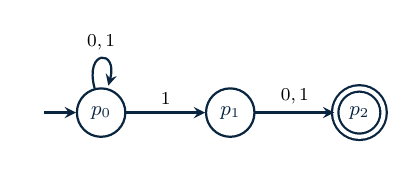
\begin{tikzpicture}[scale=0.82, every node/.style={transform shape}]
          \node[state, initial] (p0) at (0, 0) {$p_0$};
          \node[state] (p1) at (2.0, 0) {$p_1$};
          \node[state, accepting] (p2) at (4.0, 0) {$p_2$};
          
          \path (p0) edge[loop above] node{$0, 1$} (p0)
                (p0) edge node[above]{$1$} (p1)
                (p1) edge node[above]{$0, 1$} (p2);
        \end{tikzpicture}
      \end{center}
      \begin{tcolorbox}[spotlightcard]
        \cardtitle{Equivalence Theorem Preview:}
        {\scriptsize
        \textbf{Rabin \& Scott (Turing Award):} Every NFA can be converted to an equivalent DFA via the \textbf{Powerset Construction}:
        \[ L(\text{NFA}) \equiv L(\text{DFA}) \]
        }
      \end{tcolorbox}
    \end{column}
  \end{columns}
\end{frame}

% ------------------------------------------------------------------------------
% SLIDE 16: Week 2 Synthesis & Problem Set 1 Assignment
% ------------------------------------------------------------------------------
\begin{frame}{Week 2 Synthesis \& Problem Set 1}
  \framesubtitle{Mastery checklist, required readings, and milestone deliverables}
  
  \begin{columns}[T]
    \begin{column}{0.48\textwidth}
      \colheader{Week 2 Concept Checklist}
      \begin{tcolorbox}[conceptcard]
        \cardtitle{You should now be able to:}
        \begin{itemize}\setlength{\itemsep}{2pt}\scriptsize
          \item Write formal 5-tuples $M = (Q, \Sigma, \delta, q_0, F)$ without ambiguity.
          \item Construct state diagrams for substring, modulo, and divisibility patterns.
          \item Formulate computation traces and state invariants using extended $\delta^*$.
          \item Execute the Product Construction proof for Union ($\cup$) and Intersection ($\cap$).
          \item Explain the $\mathcal{O}(1)$ throughput advantages of DFAs in Zeek/Snort DPI and compiler lexers.
        \end{itemize}
      \end{tcolorbox}
    \end{column}
    
    \begin{column}{0.48\textwidth}
      \colheader{Milestone: Problem Set 1 Assigned}
      \begin{tcolorbox}[examplecard]
        \greentitle{Problem Set 1 (Due Week 3):}
        \begin{itemize}\setlength{\itemsep}{1.5pt}\scriptsize
          \item \textbf{Problem 1:} Formal DFA design for binary numbers divisible by 5.
          \item \textbf{Problem 2:} Dual parity DFA for 3-letter alphabet $\{a, b, c\}$.
          \item \textbf{Problem 3:} Formal proof that regular languages are closed under Symmetric Difference ($A \oplus B$).
        \end{itemize}
        \vspace{0.04cm}
        
        \greentitle{Required Reading:}
        {\scriptsize Sipser (3rd Ed.), \textbf{Section 1.1: Finite Automata} (pp.~31--44).}
      \end{tcolorbox}
    \end{column}
  \end{columns}
  
  \vspace{0.08cm}
  \begin{tcolorbox}[spotlightcard]
    \centering
    {\scriptsize\textbf{Office Hours:} Tuesdays \& Thursdays 14:00--16:00 GMT \;\textbar\; GIMPA School of Technology}
  \end{tcolorbox}
\end{frame}

\end{document}
